% ============================================================
% 产品说明书 — 时序数据采集与应用管理系统
% 从用户视角：这是什么、能干什么、怎么构成的
% ============================================================
\documentclass[11pt,a4paper]{ctexart}
\usepackage{xeCJK,xcolor,graphicx,float,fancyhdr,hyperref,geometry,longtable,booktabs,enumitem,caption,tikz}
\usetikzlibrary{arrows.meta,positioning,calc}
\setCJKmainfont{Microsoft YaHei}
\geometry{a4paper,margin=2.2cm}
\pagestyle{fancy}
\fancyhead[L]{时序数据采集与应用管理系统 — 产品说明书}
\fancyhead[R]{V1.0}
\fancyfoot[C]{\thepage}
\hypersetup{colorlinks=true,linkcolor=black,urlcolor=blue}

\begin{document}

\begin{center}
{\Huge\bfseries 时序数据采集与应用管理系统\\ 产品说明书}\\
{\large 从用户视角了解系统：这是什么、能干什么、怎么构成的}\\
{\large 版本 V1.0 \quad 2026-08}
\end{center}

\vspace{1em}\noindent\hrulefill\vspace{1em}

\section{产品概述}

本系统是大庆油田时序数据采集与应用管理的专用平台。一句话概括：

\begin{center}
\large\bfseries 把全油田 16 个厂、100+ 作业区、260 万+ 设备点位的数据\\自动采上来、实时算出来、一目了然呈现出来。
\end{center}

\subsection{它解决什么问题}

当前 A11 系统按"统一点位、统一频率、统一配置"运行——全油田一种节奏。但每个作业区的设备类型、工况、需求各不相同：有的需要高频采集功图、有的需要秒级异常报警、有的需要用 4G 移动网关接入。标准服务无法满足差异化需求。

本系统\textbf{不替代 A11}（A11 继续运行、原业务不受影响），而是在 A11 旁边并行一条新通道：\textbf{按每个作业区的实际需求，定制采集策略、定制流水算法、统一汇聚呈现}。

\subsection{核心能力三句话}

\begin{enumerate}[leftmargin=*]
  \item \textbf{采得全}——10+ 种工业协议（A11/Modbus/OPC DA/IEC104/MQTT）、双路采集（有线设备主动连、4G 设备桥接转发）、10 家网关厂家适配、断网自动补传
  \item \textbf{算得准}——15 种油田内置算法 + 每作业区定制注册，数据在入库前就完成计算和告警判定，不是"存完再查"
  \item \textbf{看得见}——驾驶舱大屏一眼看全油田，9 大功能模块覆盖设备管理、接入监控、算法管理、告警闭环、数据分析、可视化组态、自动化联动
\end{enumerate}

\section{系统构成：两个底座 + 插件}

本系统\textbf{不是从零开发}——是在两个成熟底座上增加油田定制插件，底座提供通用能力（MQTT Broker、数据 API、认证、存储引擎），插件提供油田专用功能。

\begin{table}[H]\centering
\caption{底座 vs 插件 —— 架构分层}
\begin{tabular}{p{3.2cm} p{5.0cm} p{5.0cm}}
\toprule
 & \textbf{边缘代理} & \textbf{边缘中枢} \\
\midrule
\textbf{底座} & dgiot\_lite (Python + Vue3) & dgaiot (Erlang 基础层) + Python 应用层 \\
\textbf{应用层} & Python: 双路采集 · 动态调频 · 断网补传 · 物模型配点 · 作业区适配 · 网关适配 & Python: 流水计算 · 告警引擎 · 数据服务 · 自动化 · 报表 \\
\textbf{高并发/状态机} & — & Erlang: dgiot MQTT · 设备影子状态机 · 协议并发 · OTP 监督树 · 本体论引擎 \\
\textbf{基础设施} & FastAPI · SQLite · 前端 25 View & PostgreSQL · TDengine · Parse · Nginx · 36 OTP \\
\textbf{部署在哪} & IO 服务器（生产网 Win2016） & openEuler/麒麟 Linux DMZ 区 \\
\textbf{数量} & 每作业区 1 台（约 200 台） & 全油田 1 套 \\
\bottomrule
\end{tabular}
\end{table}



\subsection{边缘代理 vs 边缘中枢 —— 功能边界}

\begin{table}[H]\centering
\begin{tabular}{p{3.8cm} p{5.2cm} p{5.2cm}}
\toprule
 & \textbf{边缘代理（Edge Agent）} & \textbf{边缘中枢（Edge Hub）} \\
\midrule
\textbf{部署在哪} & 作业区 IO 服务器（生产网） & DMZ 区麒麟 Linux 服务器 \\
\textbf{一句话职责} & dgiot\_lite + 插件 → 采下来、推上去 & dgaiot + 插件 → 汇起来、算出来、呈现出来 \\
\textbf{负责什么} & 协议解析 · 双路采集 · 动态调频 · 断网补传 · 设备感知 · 数据上报 & MQTT 汇聚 · 流水计算 · 告警引擎 · 混合存储 · 驾驶舱大屏 · 管理后台 \\
\textbf{不负责什么} & 不存数据 · 不算告警 · 不展示界面 & 不直接采设备 · 不做设备侧缓存 \\
\textbf{设备数量} & 每作业区 1 台，全油田约 200 台 & 全油田 1 套 \\
\textbf{对应报价} & 板块三 + 板块四（定制） & 板块一 + 板块二（部署） \\
\bottomrule
\end{tabular}
\end{table}

begin{center}	extbf{系统由两个组件构成：边缘代理（采）+ 边缘中枢（汇·算·存·展示）}end{center}



\section{边缘代理：把数据采上来}

边缘代理部署在每台作业区 IO 服务器上，与 A11 服务同机共存、互不影响。它的工作很简单：\textbf{把数据从设备上取下来，通过 MQTT 推给边缘中枢}。

\subsection{边缘代理功能清单}

\begin{table}[H]\centering
\begin{tabular}{p{3.2cm} p{8.0cm}}
\toprule
\textbf{功能} & \textbf{用户视角说明} \\
\midrule
多协议采集 & 无论是 A11 专有协议的设备、Modbus 的 RTU、还是 OPC DA 的 DCS 控制站——一个代理全部能接 \\
双路采集 & 固定 IP 的有线设备：系统主动连接去取；4G 移动网关的动态 IP 设备：系统桥接到原地址，复制一份数据、原样转发给 A11（A11 不受影响） \\
设备自动发现 & 新设备接入、旧设备下线——代理自动感知，不需要人工登记 \\
动态调频 & 平时按正常频率采；出现异常自动加密到秒级；夜间低峰自动降频省资源 \\
断网补传 & 网络断了数据存在本地；网络恢复后按时间顺序补传上去，不丢、不重 \\
物模型配点 & 油水井 G1-G8 标准物模型（64 点/井），一键生成点位表，不用手工配 \\
10 家网关适配 & 宏电、映翰通、亿帆、有人、四信、移远、合宙、中易云、万物纵横、莱特——全部适配 \\
\bottomrule
\end{tabular}
\end{table}

\section{边缘中枢：汇·算·存·展示}

边缘中枢部署在 DMZ 区的麒麟 Linux 服务器上。它接收全油田所有边缘代理推送的数据，完成汇聚、计算、存储和展示。

\subsection{边缘中枢功能清单}

\begin{table}[H]\centering
\begin{tabular}{p{3.0cm} p{8.2cm}}
\toprule
\textbf{功能} & \textbf{用户视角说明} \\
\midrule
MQTT 消息汇聚 & 同时接收 200+ 台 IO 服务器的实时数据推送，千万级并发能力 \\
流水计算引擎 & 15 种油田内置算法（工况诊断/预警/统计类）开箱即用；每个作业区可注册自己的定制算法，数据入库前就完成计算和告警判定 \\
告警引擎 & 四级告警（严重/重要/一般/提示），发现后自动通知（大屏弹窗/短信/电话），逐级升级直到有人确认处理，全程留痕 \\
混合存储 & 时序数据用 TDengine（快）、资产台账用 PostgreSQL（稳）、边缘降级用 SQLite（不丢），冷热数据自动分层 \\
驾驶舱大屏 & 深色底大屏，中间是采集链路拓扑图（作业区→设备→链路，绿色正常/黄色降频/红色离线），左边 KPI 卡片，右边告警滚动 \\
管理后台 & 9 大功能模块：设备管理/设备接入/算法管理/告警中心/数据服务/可视化/自动化/系统管理 \\
\bottomrule
\end{tabular}
\end{table}

\begin{figure}[H]\centering
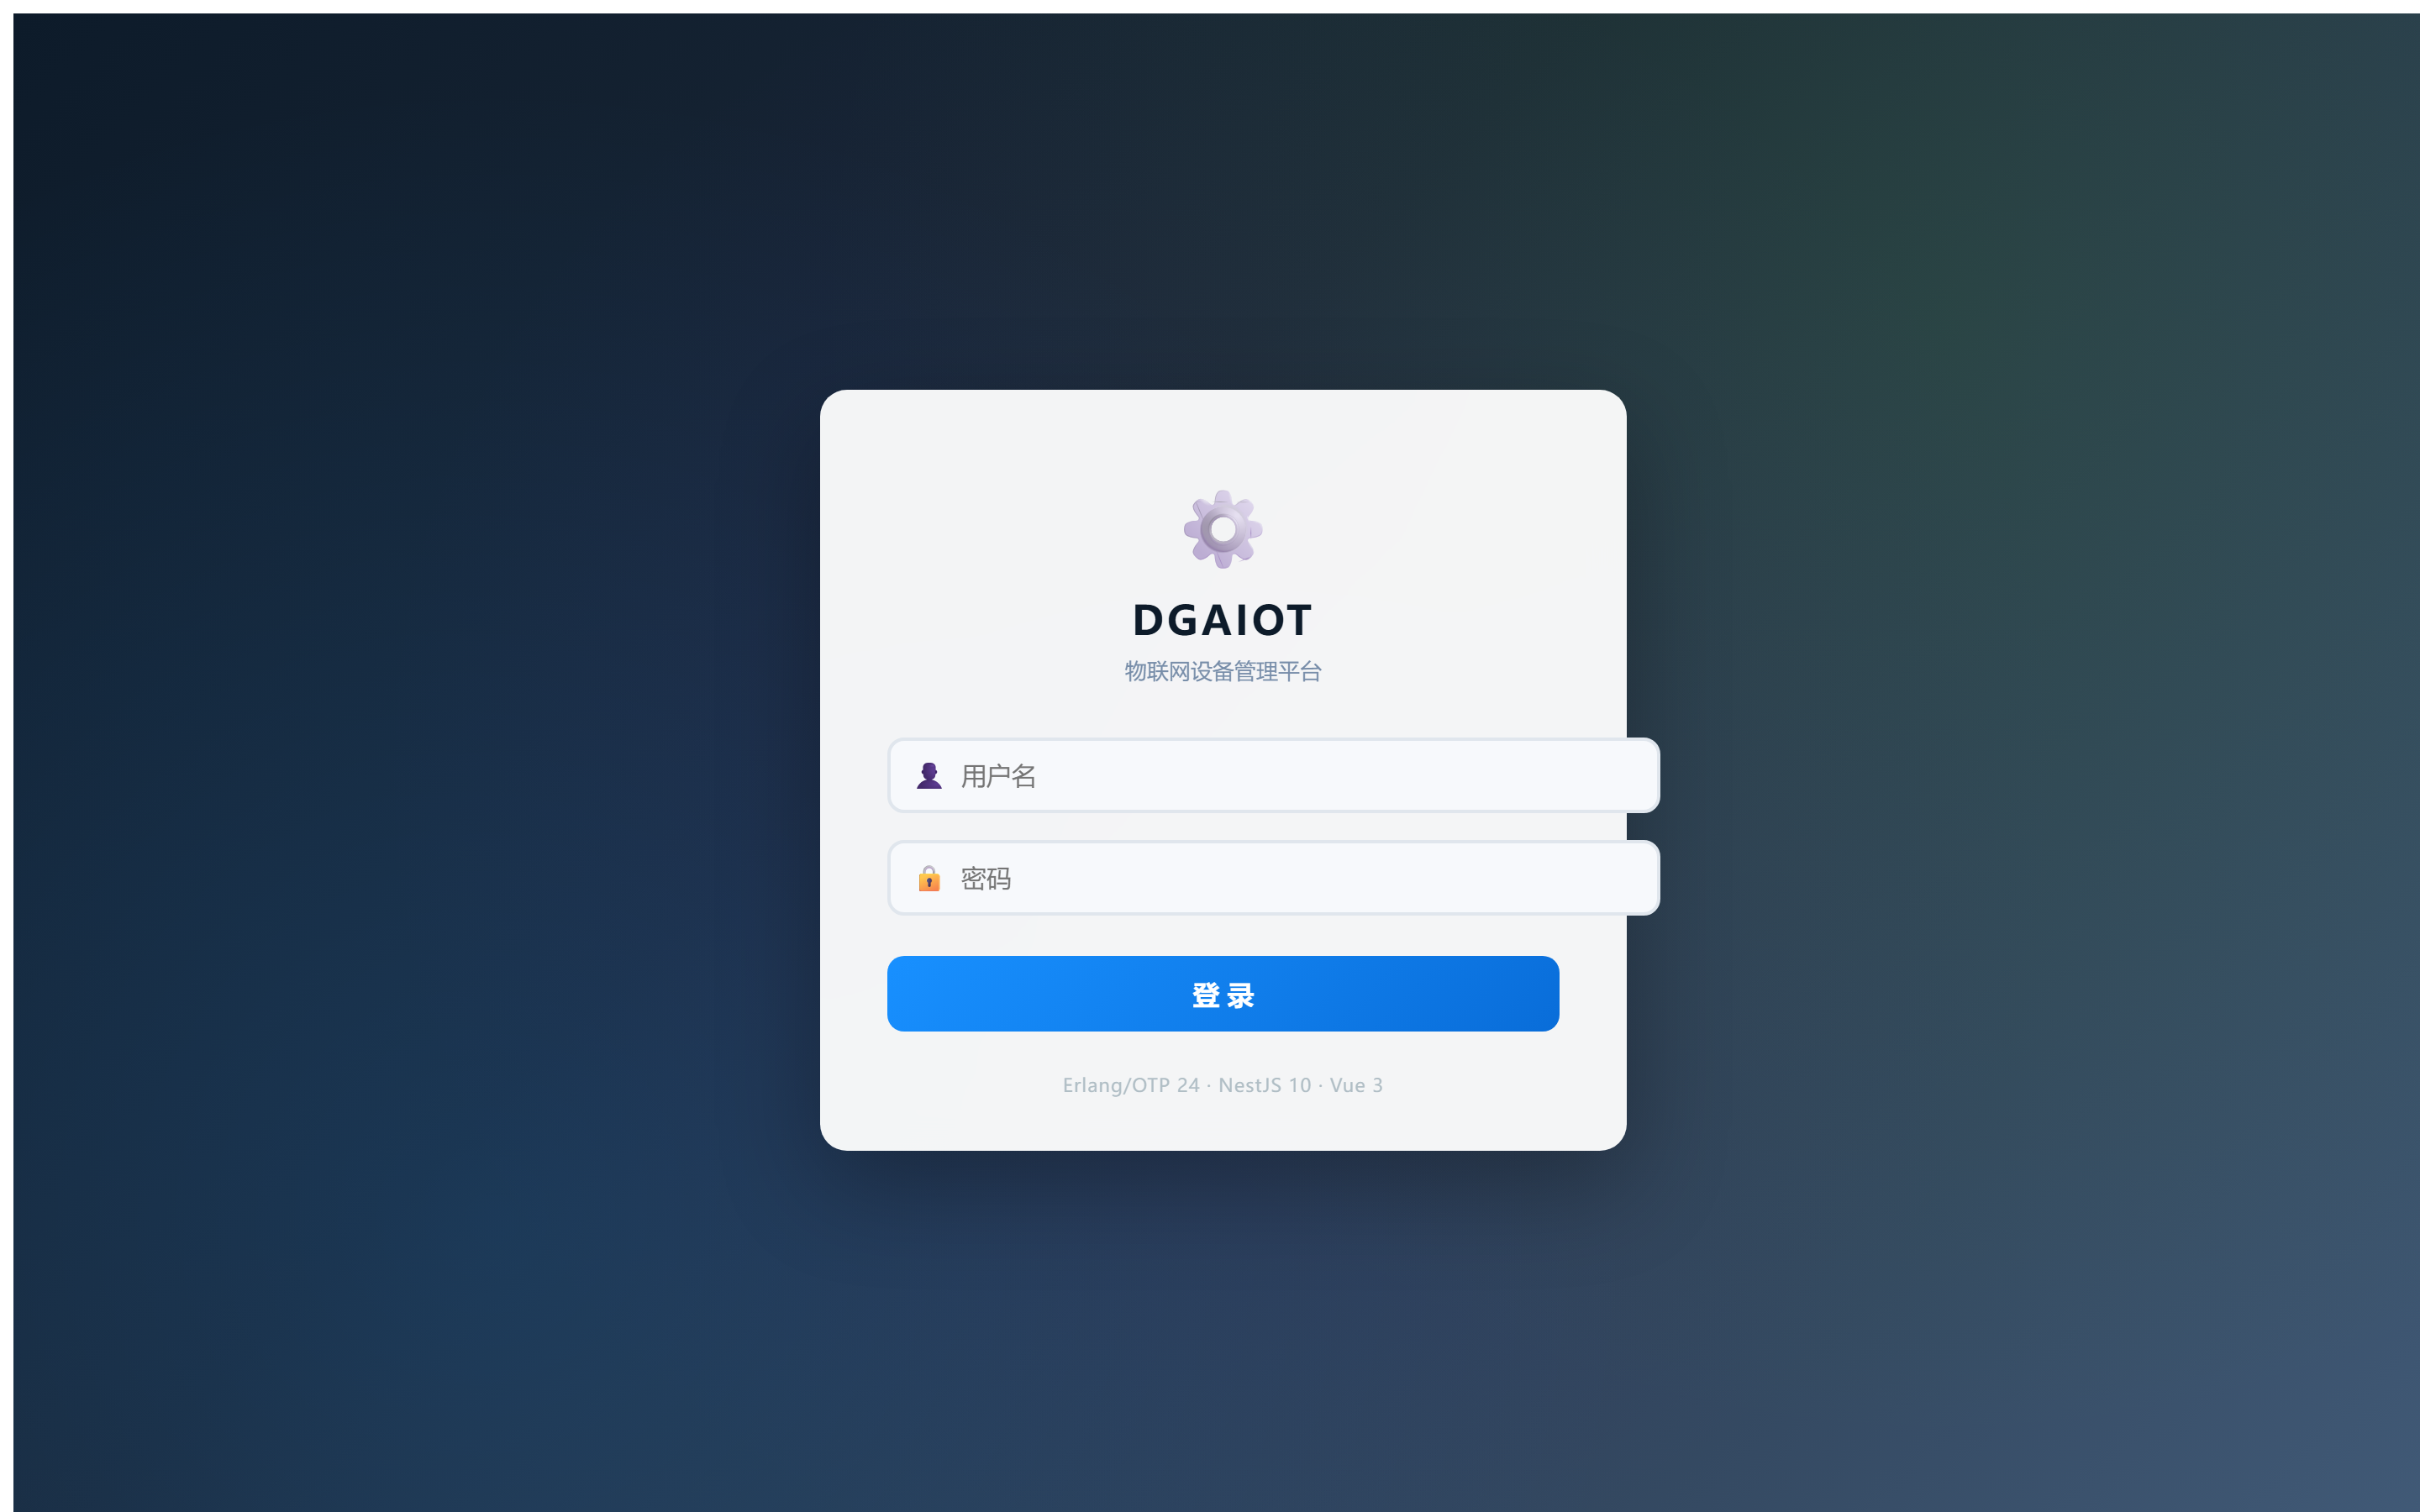
\includegraphics[width=0.92\textwidth]{实际运行-dashboard.png}
\caption{系统实际运行界面——566 台设备在线，9 模块导航}
\end{figure}

\section{管理后台：9 大功能模块}

打开系统后，左侧导航有 9 个模块，每个模块对应一个用户关心的实际问题：

\begin{table}[H]\centering
\begin{tabular}{p{2.4cm} p{3.2cm} p{7.6cm}}
\toprule
\textbf{模块} & \textbf{回答什么问题} & \textbf{能做什么} \\
\midrule
① 驾驶舱 & 一切正常吗？ & 大屏看板：KPI 卡片、链路拓扑、告警滚动、采集频率趋势——全油田 10 秒看懂 \\
② 设备管理 & 资产管住了吗？ & 设备台账（全油田设备清单）、五态生命周期（在线/离线/未激活/异常/冻结）、6 页签详情、物模型一键配点 \\
③ 设备接入 & 数据都接上来了吗？ & 每台终端链路状态、采集频率、断网补传进度条、网关在线地图 \\
④ 算法管理 & 算法注册了几个？ & 15 种内置算法库、作业区定制注册制、A/B 对比、逐井调优、可视化规则编排 \\
⑤ 告警中心 & 异常有人管吗？ & 四级告警列表、工单流转闭环（发现→确认→处置→归档）、升级链、通知记录 \\
⑥ 数据服务 & 数据取得出吗？ & 报表（日/月/年）、曲线回放（时间轴拖拽）、健康日报自动生成、REST API \\
⑦ 可视化 & 结构看清楚了吗？ & 采集链路拓扑图、拖拽式仪表盘组态、GIS 地图层级下钻 \\
⑧ 自动化 & 能自己跑吗？ & 规则联动（触发→判定→执行）、场景编排（批量下发/定时巡检）、设备影子 \\
⑨ 系统管理 & 谁在看、谁动过？ & 角色权限（领导/调度/运维三种视图）、审计日志、国密加密、信创适配 \\
\bottomrule
\end{tabular}
\end{table}

\section{部署拓扑}

begin{center}	extbf{系统部署拓扑：边缘代理在生产网采数据，MQTT 推送到 DMZ 区边缘中枢完成计算存储展示}end{center}



\section{关键数字}

\begin{table}[H]\centering
\begin{tabular}{p{3.5cm} p{3.0cm} p{5.0cm}}
\toprule
\textbf{指标} & \textbf{数值} & \textbf{说明} \\
\midrule
覆盖范围 & 16 厂 · 100+ 作业区 & 全油田 \\
设备点位 & 260 万+ & 全量采集 \\
单作业区测点 & ~4.7 万 & 第四作业区实测 \\
并发接入 & 200+ IO 服务器 & 每作业区 1 台 \\
内置算法 & 15 种 & 工况诊断/预警/统计 \\
采集协议 & 10+ 种 & A11/Modbus/OPC DA/IEC104/MQTT/HTTP \\
网关厂家 & 10 家 & 全部适配 \\
系统界面 & 9 大模块 & 管理后台 \\
\bottomrule
\end{tabular}
\end{table}

\vspace{1em}\noindent\hrulefill
\begin{center}\small
编制单位：迪格(杭州)物联科技有限公司 \quad 2026-08 \quad 配套：报价书、报价表 V10、功能边界清单
\end{center}

\end{document}
